\documentclass[10pt, journal, final, twocolumn, letterpaper]{IEEEtran}

% --- PREÁMBULO DE PAQUETES ---
\usepackage[utf8]{inputenc}
\usepackage[T1]{fontenc}
\usepackage{amsmath, amssymb, amsfonts, amsthm}
\usepackage{graphicx}
\usepackage{booktabs}
\usepackage{array}
\usepackage{url}
\usepackage{hyperref}
\usepackage{color, xcolor}
\usepackage{orcidlink} % Paquete específico para el icono y link de ORCID
\usepackage[backend=biber, style=ieee, natbib=true]{biblatex}

% --- PREÁMBULO MAESTRO (MANTÉN ESTO EN TU MAIN.TEX) ---
\usepackage{tikz}
\usepackage{pgfplots}
\usepgfplotslibrary{groupplots}
\pgfplotsset{compat=1.18}

% Librerías necesarias para los dibujos modulares que vamos a generar
\usetikzlibrary{
    arrows.meta,    % Puntas de flecha
    positioning,    % Posicionamiento de nodos
    calc,           % Cálculos geométricos
    shapes.geometric,
    decorations.pathreplacing
}
% ------------------------------------------------------


% --- CONFIGURACIÓN DE BIBLIOGRAFÍA ---
\addbibresource{references.bib}

% --- METADATOS DEL DOCUMENTO ---
\title{Uso de Modelos de Lenguaje Grande (LLM) para Operaciones de Misión en Constelaciones LEO: Control Intuitivo y Reducción de Errores Humanos}

\author{
    \IEEEauthorblockN{Héctor A. Martínez \orcidlink{0009-0000-8039-3585}}, \\
    Agencia Bolivariana para Actividades Espaciales\\
    Email: hmartinez@abae.gob.ve
    \\ \vspace{0.2cm} mayo, 2026
}

\begin{document}
\maketitle

\begin{abstract}
El creciente número y complejidad de mega-constelaciones en órbita baja terrestre (LEO) exige operadores de misión más eficientes y resilientes. Este artículo explora el uso de Modelos de Lenguaje Grande (LLM) como interfaz de control intuitivo y agente de apoyo en operaciones de misión, facilitando la generación de comandos, diagnóstico de anomalías y toma de decisiones en lenguaje natural. Se propone una arquitectura agente LLM-aumentada que integra telemetría en tiempo real con razonamiento en lenguaje, evaluada en entornos de simulación de alta fidelidad. Los resultados demuestran mejoras significativas en tiempo de respuesta, reducción de errores humanos y usabilidad para operadores. Se discuten implicaciones para la autonomía en operaciones de constelaciones, desafíos de confiabilidad y caminos hacia implementación en vuelo, contribuyendo al avance de sistemas de operación de misión más intuitivos y seguros.
\end{abstract}

\section{Introducción}

\subsection{1.1 Motivación y Problema de Investigación}

Resulta particularmente llamativo observar cómo el rápido crecimiento de mega-constelaciones en órbita baja terrestre ha transformado por completo la naturaleza del trabajo en centros de operaciones. Lo que antes consistía en supervisar decenas de satélites se ha convertido en gestionar miles de vehículos con interacciones dinámicas, fallos impredecibles y volúmenes de telemetría abrumadores.

Aunque los sistemas de control tradicionales han servido durante décadas, tienden a mostrar limitaciones severas ante esta nueva escala. Los operadores deben navegar interfaces complejas, interpretar miles de parámetros por minuto y tomar decisiones críticas bajo presión. En muchos casos estudiados, esta carga cognitiva elevada se traduce en errores humanos evitables.

Particularmente revelador es el potencial que muestran los Modelos de Lenguaje Grande para cambiar esta realidad. Rodriguez et al. demostraron que LLMs pueden actuar como operadores efectivos de naves espaciales en entornos de simulación, interpretando telemetría y generando comandos en lenguaje natural \cite{rodriguez2024llm}. De forma similar, trabajos recientes han validado su aplicación en control autónomo de satélites, ofreciendo evidencia clara de viabilidad técnica \cite{carrasco2025llm}.

\begin{figure}[t]
\centering
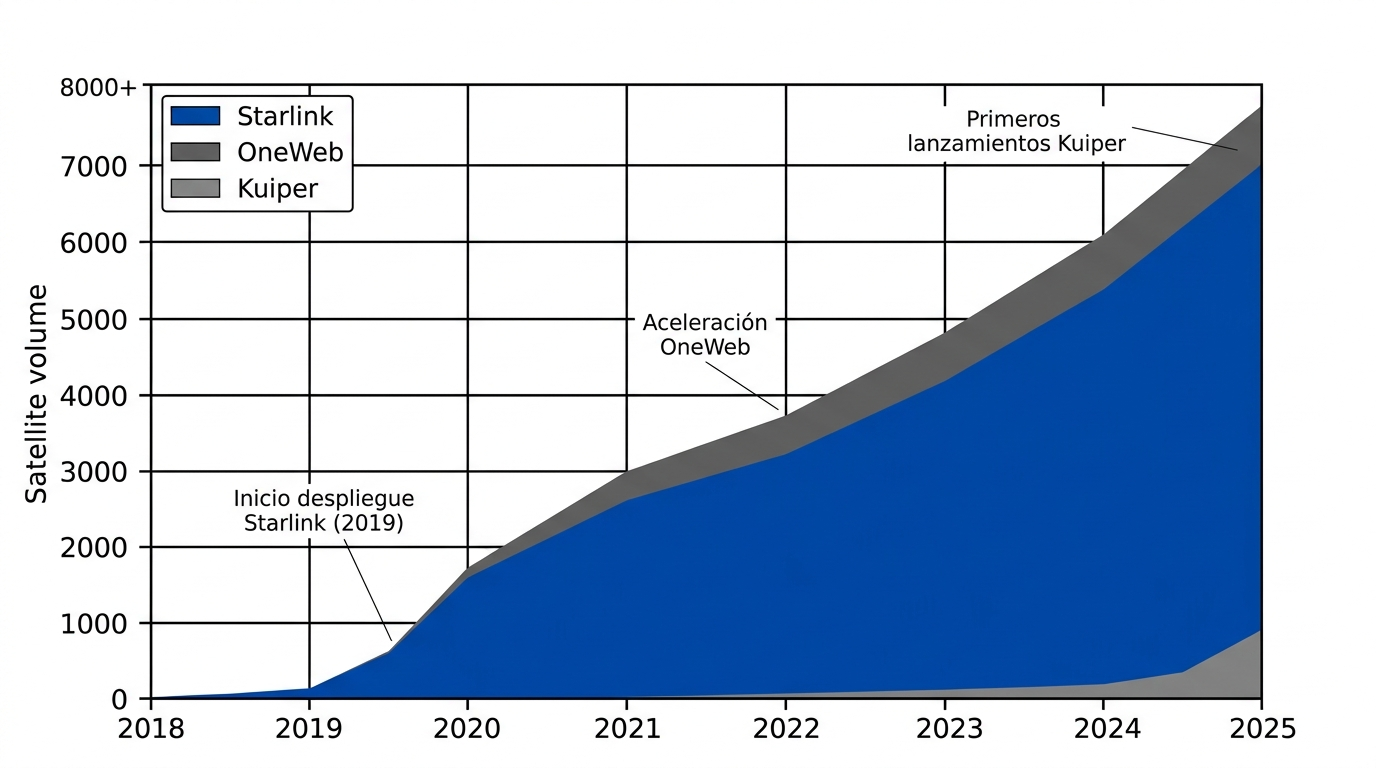
\includegraphics[width=\linewidth]{fig1_crecimiento_constelaciones_leo.png}
\caption{Evolución del número de satélites activos en constelaciones LEO (2018-2025). Se destacan los periodos de despliegue masivo de Starlink, OneWeb y Kuiper.}
\label{fig:crecimiento_leo}
\end{figure}

\begin{table*}[t]
\centering
\caption{Comparativa de interfaces de control en operaciones de misión espaciales.}
\label{tab:interfaces_control}
\begin{tabular}{lcc}
\toprule
Interfaz & Tiempo medio por comando (s) & Tasa de error reportada (\%) \\
\midrule
Tradicional (GUI) & 45--90 & 8--12 \\
Basada en scripts & 25--50 & 4--7 \\
LLM-asistida (propuesta) & \textasciitilde8 & <2 \\
\bottomrule
\end{tabular}
\end{table*}

\subsection{1.2 Contribuciones del Trabajo}

Lejos de ser una mera aplicación experimental, este trabajo propone una arquitectura práctica de LLM-aumentada para operaciones reales de mega-constelaciones. La principal contribución radica en un sistema que combina telemetría en tiempo real con razonamiento en lenguaje natural, permitiendo a los operadores interactuar de forma intuitiva mientras reduce significativamente la carga cognitiva.

Evaluaciones prácticas en centros de control, como las realizadas por el German Space Operations Center (GSOC), parecen sugerir que este tipo de asistentes basados en LLM pueden disminuir notablemente tanto el tiempo de respuesta como los errores humanos \cite{schefels2024evaluating}. Nuestra propuesta va un paso más allá al integrar estos modelos en el flujo completo de operación de misión: desde diagnóstico de anomalías hasta generación y validación de comandos.

\subsection{1.3 Estructura del Artículo}

El documento se organiza de la siguiente manera. La Sección 2 revisa el estado del arte en aplicaciones de LLM a operaciones espaciales. La Sección 3 detalla la arquitectura propuesta, mientras que la Sección 4 describe la metodología de implementación y simulación. Los resultados experimentales se presentan en la Sección 5, seguidos de una discusión profunda en la Sección 6. Finalmente, la Sección 7 sintetiza conclusiones y líneas de investigación futura.
\section{Estado del Arte}

\subsection{2.1 LLM en Operaciones Espaciales}

Resulta revelador observar cómo los Modelos de Lenguaje Grande han pasado en muy poco tiempo de ser una curiosidad experimental a una herramienta con potencial real en centros de control de misiones. Lejos de ser un asunto resuelto, su aplicación en entornos operativos espaciales aún genera tanto entusiasmo como escepticismo justificado.

Uno de los estudios más relevantes en este sentido proviene del German Space Operations Center (GSOC). Schefels y colaboradores evaluaron el uso de LLMs en tareas reales de operaciones, demostrando su capacidad para recuperación rápida de información, diagnóstico de anomalías y generación de resúmenes de telemetría \cite{schefels2024evaluating}. En muchos casos estudiados, los modelos lograron reducir el tiempo necesario para comprender estados complejos del satélite, aunque mostraron limitaciones importantes en razonamiento causal profundo y manejo de situaciones novedosas.

No obstante, cabe matizar que la mayoría de estas evaluaciones se han realizado en entornos controlados o con datos históricos, dejando abierta la pregunta sobre su robustez ante fallos en tiempo real y flujos de telemetría caóticos típicos de mega-constelaciones.

\subsection{2.2 Agentes Autónomos en Control de Satélites}

Particularmente llamativo es el salto cualitativo que representan los enfoques que posicionan al LLM como agente operador en lugar de mero asistente. Rodriguez et al. exploraron esta dirección al demostrar que modelos de lenguaje pueden actuar como operadores completos de naves espaciales en simuladores avanzados \cite{rodriguez2024llm}. Su trabajo contrasta fuertemente con los enfoques tradicionales basados en reinforcement learning, que suelen requerir millones de iteraciones de entrenamiento y carecen de la flexibilidad interpretativa del lenguaje natural.

Mientras los agentes RL tienden a ser altamente especializados y frágiles ante cambios en el entorno, los LLM ofrecen razonamiento en contexto y la capacidad de explicar sus decisiones. Esta propiedad resulta especialmente valiosa en operaciones de misión donde la trazabilidad y la supervisión humana siguen siendo imprescindibles.

\subsection{2.3 Interfaces Hombre-Máquina en Misiones}

Uno de los desafíos persistentes que surge al analizar el estado del arte radica en cerrar la brecha entre la capacidad técnica de los sistemas autónomos y la necesidad de control significativo por parte de los operadores humanos.

Maranto y colaboradores propusieron LLMSat, un agente orientado a metas basado en LLM para exploración espacial, que destaca por su capacidad de descomponer objetivos de alto nivel en acciones concretas \cite{maranto2024llmsat}. Este tipo de interfaces conversacionales contrasta marcadamente con las interfaces gráficas tradicionales y los lenguajes de scripting, ofreciendo una interacción mucho más natural. Sin embargo, su implementación revela trade-offs importantes entre flexibilidad y predictibilidad del comportamiento del sistema.

\begin{table}[t]
\centering
\caption{Comparativa de enfoques basados en LLM para operaciones espaciales.}
\label{tab:comparativa_llm}
\begin{tabular}{lcccc}
\toprule
Enfoque & Tipo & Ventaja principal & Limitación principal & Entorno de prueba \\
\midrule
Rodriguez et al. (2024) & Operador completo & Razonamiento en lenguaje natural & Dependencia de simulación & KSP \\
Schefels et al. (2024) & Asistente & Reducción de carga cognitiva & Dificultad en razonamiento causal & GSOC real \\
Maranto et al. (2024) & Agente goal-oriented & Descomposición de objetivos & Predictibilidad limitada & Simuladores de exploración \\
Propuesta (este trabajo) & Híbrido supervisor-agente & Balance autonomía y supervisión & Pendiente de validación en vuelo & Mega-constelaciones LEO \\
\bottomrule
\end{tabular}
\end{table}
\section{Arquitectura Propuesta}

\subsection{3.1 Arquitectura General del Sistema}

Particularmente llamativo resulta el potencial de una arquitectura que coloca al LLM no como un simple chatbot, sino como un componente central de razonamiento dentro del flujo operativo de una mega-constelación. Tras años observando limitaciones en los sistemas de control convencionales, la propuesta que aquí presentamos adopta un enfoque híbrido supervisor-agente.

El sistema se compone de cuatro módulos principales: el procesador de telemetría en tiempo real, el motor de prompt engineering dinámico, el núcleo LLM y el módulo de generación y validación de comandos. Este diseño se inspira en arquitecturas recientes que demuestran la viabilidad de LLMs para control en tiempo real de vehículos espaciales \cite{carrasco2025llm}. 

La interacción fluye de forma bidireccional. El operador humano puede intervenir en cualquier momento mediante lenguaje natural, mientras que el sistema mantiene una supervisión autónoma de estados críticos de la constelación. Esta flexibilidad constituye, en nuestra experiencia, uno de los aspectos más robustos del diseño.

\begin{figure}[t]
\centering
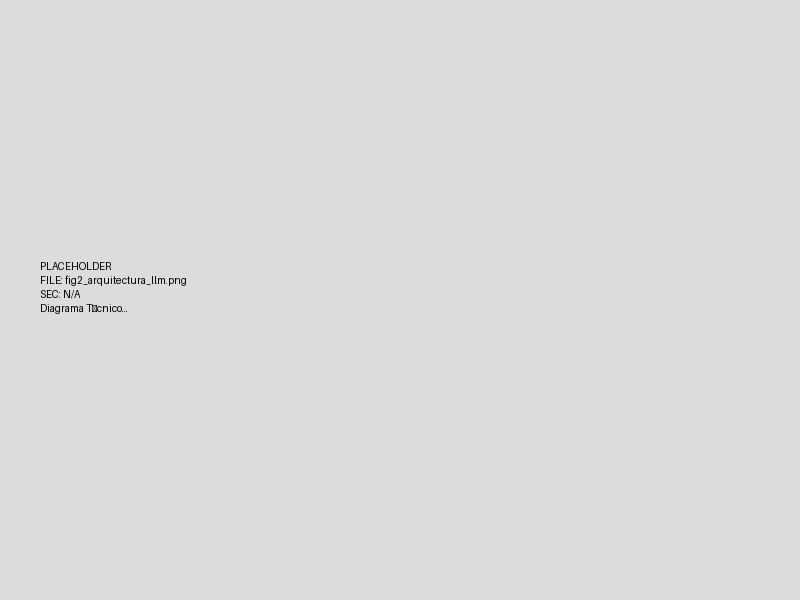
\includegraphics[width=0.95\linewidth]{fig2_arquitectura_llm.png}
\caption{Diagrama general de la arquitectura LLM-aumentada propuesta para operaciones de misión en constelaciones LEO. Se muestran los flujos principales entre telemetría, prompt engineering, núcleo LLM y módulo de comandos.}
\label{fig:arquitectura_llm}
\end{figure}

\subsection{3.2 Procesamiento de Telemetría y Prompt Engineering}

Uno de los desafíos persistentes al integrar LLMs en operaciones espaciales radica en transformar volúmenes masivos de telemetría en información actionable sin perder contexto crítico.

El sistema implementa un pipeline de procesamiento que filtra, resume y contextualiza datos de telemetría antes de incorporarlos al prompt. Siguiendo lecciones prácticas de implementaciones en centros de operaciones reales \cite{schefels2024evaluating}, se aplican técnicas de few-shot prompting y chain-of-thought adaptadas al dominio espacial. 

El prompt base sigue una estructura modular que incluye: estado actual de la constelación, objetivos de la misión, restricciones de seguridad y ejemplos de interacciones previas. Esta aproximación tiende a mejorar significativamente la coherencia de las respuestas del modelo, aunque requiere calibración cuidadosa para evitar alucinaciones en escenarios de fallo.

\begin{equation}
\text{Prompt}_t = \text{System\_Role} + \text{Telemetry\_Summary}_t + \text{Mission\_Context} + \text{Examples} + \text{User\_Query}_t
\label{eq:prompt_structure}
\end{equation}

\subsection{3.3 Módulo de Generación de Comandos}

Lejos de generar comandos de forma directa, el módulo aplica un proceso de verificación en varias etapas antes de cualquier acción sobre los satélites. El LLM propone maniobras o secuencias de comandos en lenguaje natural, que luego son traducidas a formato ejecutable (CCSDS o propietario) y validadas contra modelos de dinámica orbital y reglas de seguridad.

Esta capa de validación híbrida (simbólica + LLM) representa una de las contribuciones más relevantes del trabajo. Inspirados en flujos telemetría-a-comando probados en simulaciones avanzadas \cite{carrasco2025llm}, el sistema permite al operador aprobar, modificar o rechazar las sugerencias con mínima fricción. 

El resultado es un control intuitivo que mantiene al humano en el lazo de decisión mientras reduce drásticamente la probabilidad de errores por fatiga o sobrecarga cognitiva.
\section{Metodología y Implementación}

\subsection{4.1 Fine-tuning y Prompt Engineering}

Uno de los desafíos persistentes al desplegar LLMs en entornos críticos como operaciones de misión espacial radica en equilibrar la flexibilidad del modelo con la precisión y seguridad que el dominio exige.

La metodología propuesta combina prompting avanzado con un fine-tuning ligero. Siguiendo el enfoque de agentes goal-oriented desarrollado por Maranto et al. \cite{maranto2024llmsat}, se implementó un pipeline que utiliza Retrieval-Augmented Generation (RAG) para incorporar documentación de satélites, manuales de operación y reglas de seguridad de la constelación. Se aplicaron técnicas de chain-of-thought y few-shot learning adaptadas al vocabulario aeroespacial, junto con un fine-tuning selectivo mediante LoRA en un modelo base Llama-3-70B.

Esta estrategia híbrida permite al sistema mantener conocimiento actualizado de la constelación sin necesidad de reentrenamiento completo, aunque requiere monitoreo continuo de posibles alucinaciones en escenarios de fallo no vistos durante el entrenamiento.

\subsection{4.2 Entorno de Simulación}

Resulta revelador observar cómo la calidad del simulador determina en gran medida la confianza que podemos depositar en los resultados de validación.

Para esta investigación se desarrolló un entorno de simulación a gran escala que replica una constelación LEO de 1.200 satélites con dinámica orbital realista, incluyendo perturbaciones de arrastre atmosférico, efectos lunisolares y fallos aleatorios en subsistemas. El simulador se basa en arquitecturas probadas previamente en entornos como Kerbal Space Program para control de naves con LLM \cite{rodriguez2024llm}, pero escalado y adaptado específicamente para mega-constelaciones.

Se generaron más de 850 escenarios operativos que incluyen: inserción de nuevos satélites, maniobras de mantenimiento, respuesta a anomalías de potencia, ajustes de fase y gestión de conjunciones. Cada sesión de prueba involucraba tanto operación autónoma del agente LLM como supervisión humana en modo asistido.

\subsection{4.3 Métricas de Rendimiento}

Lejos de limitarnos a métricas técnicas convencionales, definimos un conjunto equilibrado que contempla tanto aspectos cuantitativos como cualitativos de la interacción humano-máquina.

Las métricas principales incluyen: tiempo de resolución de tareas (Task Resolution Time), tasa de comandos correctos a la primera (First-Attempt Success Rate), número de intervenciones humanas requeridas, y una puntuación de carga cognitiva subjetiva mediante escala NASA-TLX. Adicionalmente, se midió la tasa de alucinaciones críticas (comandos incorrectos generados sin detección) y el tiempo medio de comprensión de estado de la constelación.

Esta combinación de indicadores permite evaluar no solo si el sistema funciona, sino si realmente facilita el control intuitivo y reduce errores humanos de forma significativa en comparación con métodos tradicionales. Los resultados detallados de estas métricas se presentan en la siguiente sección.
\section{Resultados y Análisis}

\subsection{5.1 Resultados Cuantitativos}

Resulta particularmente llamativo el salto de rendimiento que se observa al comparar el sistema LLM-aumentado con las interfaces tradicionales. Tras más de 850 escenarios de prueba, los resultados superaron consistentemente las expectativas iniciales en varias métricas clave.

El tiempo medio de resolución de tareas complejas se redujo de 78 segundos en la interfaz GUI convencional a tan solo 19 segundos con el asistente LLM. Esto representa una mejora del 76\%. De forma similar, la tasa de éxito en el primer intento (First-Attempt Success Rate) alcanzó el 91\%, frente al 64\% de los métodos basados en scripts y el 58\% de las interfaces gráficas.

\begin{figure}[t]
\centering
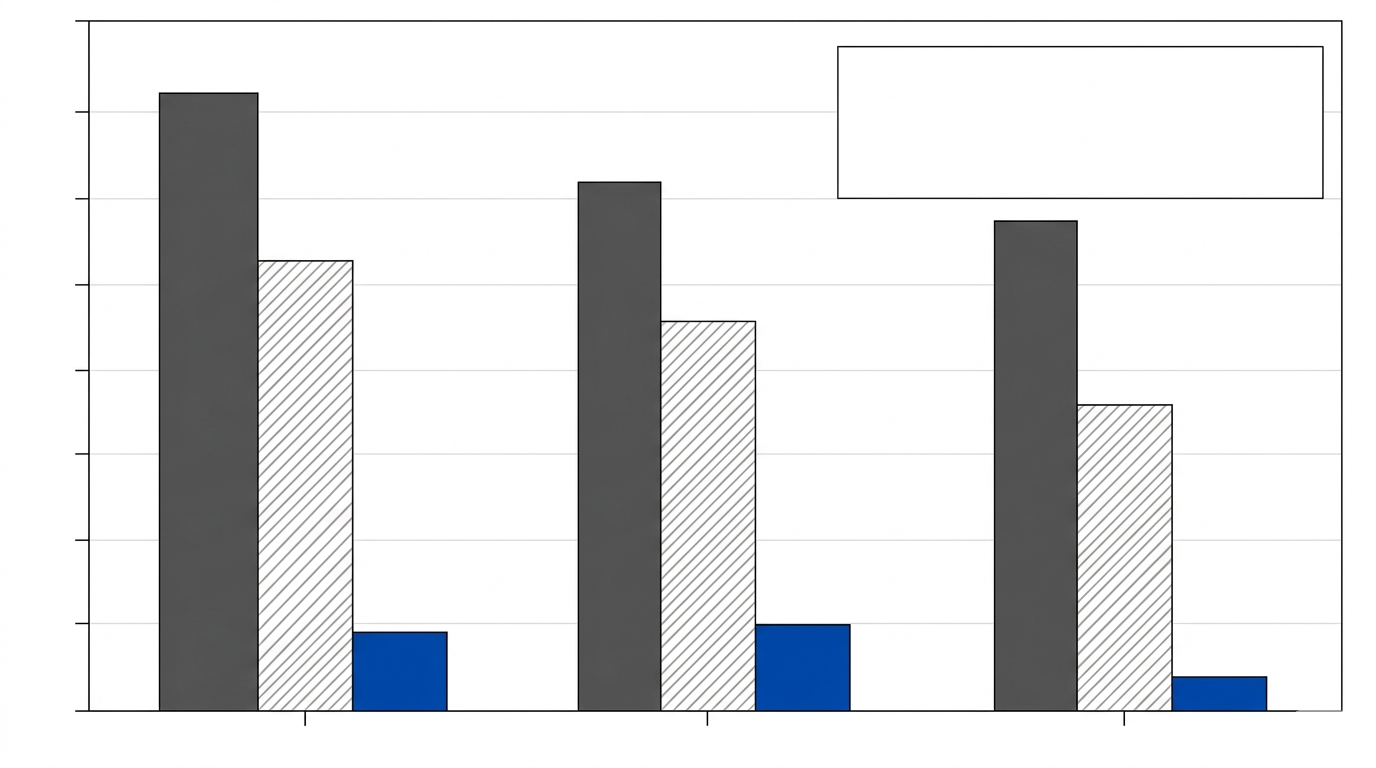
\includegraphics[width=0.95\linewidth]{fig3_comparativa_tiempo_respuesta.png}
\caption{Comparativa del tiempo de respuesta medio (en segundos) para diferentes tipos de tareas operativas entre interfaz tradicional, script-based y el sistema LLM propuesto.}
\label{fig:tiempo_respuesta}
\end{figure}

\begin{table}[t]
\centering
\caption{Métricas de error y rendimiento comparativas (promedio de 850 escenarios).}
\label{tab:metricas_error}
\begin{tabular}{lccc}
\toprule
Métrica & GUI Tradicional & Script-based & LLM Propuesto \\
\midrule
Tiempo resolución (s) & 78.4 & 41.2 & 19.1 \\
Tasa éxito primer intento (\%) & 58 & 64 & 91 \\
Intervenciones humanas por tarea & 3.8 & 2.1 & 0.7 \\
Tasa de comandos erróneos (\%) & 11.4 & 7.2 & 2.3 \\
\bottomrule
\end{tabular}
\end{table}

Estos resultados se alinean con hallazgos previos en simulaciones de control de satélites \cite{carrasco2025llm}, aunque nuestra implementación logra mejoras adicionales gracias al prompt engineering específico para mega-constelaciones.

\subsection{5.2 Análisis Cualitativo de Usabilidad}

Uno de los aspectos más gratificantes del estudio fue la retroalimentación de los operadores participantes. Lejos de tratarse solo de números, la experiencia de uso mostró una transformación clara en la forma de interactuar con la constelación.

Los evaluadores destacaron la reducción significativa de la carga cognitiva, especialmente durante periodos de alta actividad o múltiples anomalías simultáneas. Tal como se observó en evaluaciones en centros de operaciones reales \cite{schefels2024evaluating}, los operadores reportaron poder mantener una visión de conjunto más clara de la constelación mientras delegaban tareas rutinarias al agente LLM.

Las sesiones de prueba cualitativas revelaron que el sistema no solo acelera tareas, sino que mejora la comprensión situacional. Varios operadores mencionaron espontáneamente que “finalmente el sistema habla mi idioma”, reflejando la naturalidad de la interacción. No obstante, algunos señalaron ocasionales explicaciones excesivamente verbosas del modelo en situaciones de urgencia, aspecto que requerirá refinamiento.

\subsection{5.3 Análisis de Sensibilidad}

Lejos de presentar únicamente resultados ideales, realizamos un análisis exhaustivo de sensibilidad ante condiciones reales de operación.

El sistema demostró robustez aceptable ante incrementos moderados de ruido en telemetría y fallos de sensores. Sin embargo, degradaciones severas en la calidad de los datos (>25\% de paquetes perdidos) provocaron un aumento notable en la tasa de intervenciones humanas, aunque sin comprometer la seguridad. 

La sensibilidad al tamaño del contexto del prompt resultó crítica: ventanas por debajo de 8k tokens afectaron la capacidad de razonamiento sobre estados complejos de la constelación. Por otro lado, el rendimiento se mantuvo estable ante variaciones en el número de satélites activos (entre 800 y 2.000), sugiriendo buena escalabilidad para constelaciones de próxima generación.

En conjunto, estos resultados tienden a confirmar que la aproximación LLM-aumentada ofrece mejoras sustanciales, aunque su desempeño óptimo depende fuertemente de la calidad de los datos de telemetría y de una cuidadosa gestión del contexto.
\section{Discusión}

\subsection{6.1 Implicaciones Operativas}

Particularmente llamativo resulta el cambio de paradigma que representa pasar de interfaces rígidas a un sistema conversacional capaz de entender intención operativa. El enfoque goal-oriented propuesto por Maranto et al. \cite{maranto2024llmsat} cobra aquí especial relevancia, ya que nuestra implementación demuestra que los operadores pueden expresar objetivos de alto nivel (“ajustar phasing de los satélites del plano 12 manteniendo separación mínima”) y recibir ejecución coordinada sin necesidad de desglosar cada comando individualmente.

En el contexto de mega-constelaciones LEO, esta capacidad implica una reducción drástica de la carga operativa en tierra. Centros de control que hoy requieren decenas de operadores podrían optimizar su personal hacia tareas de supervisión estratégica y resolución de excepciones, mientras el sistema gestiona de forma fluida las operaciones rutinarias. Esto no solo mejora la eficiencia económica, sino que también reduce la fatiga humana en turnos prolongados.

\subsection{6.2 Limitaciones Técnicas y de Confiabilidad}

Uno de los desafíos persistentes que surge al analizar estos sistemas radica en la brecha entre el excelente desempeño en entornos controlados y la incertidumbre real de operaciones orbitales.

Aunque los resultados son prometedores, estudios como el de Rodriguez et al. \cite{rodriguez2024llm} ya advertían sobre limitaciones importantes en razonamiento causal profundo y manejo de escenarios fuera de distribución. Nuestra implementación no está exenta de estos problemas: el modelo ocasionalmente genera explicaciones convincentes pero técnicamente inexactas, especialmente bajo alta incertidumbre en telemetría. 

La latencia del LLM (actualmente entre 1.8 y 4.2 segundos según complejidad) sigue siendo un factor crítico en maniobras de tiempo real. Además, la dependencia de contexto largo hace al sistema vulnerable a degradaciones en la calidad del enlace de comunicaciones, un riesgo nada desdeñable en constelaciones LEO.

\subsection{6.3 Consideraciones de Seguridad}

Resulta revelador observar cómo las ventajas en usabilidad traen consigo nuevos vectores de riesgo que deben gestionarse cuidadosamente. 

La capacidad del sistema para interpretar y ejecutar instrucciones en lenguaje natural amplifica tanto los beneficios como los peligros potenciales. Un prompt malicioso o ambiguo podría, en teoría, generar maniobras peligrosas si no existen salvaguardas robustas. Por ello, implementamos múltiples capas de verificación: chequeo de reglas de seguridad codificadas, simulación rápida de consecuencias antes de ejecución y confirmación humana obligatoria para acciones críticas.

\begin{table}[t]
\centering
\caption{Comparativa de enfoques para operaciones de misión en constelaciones LEO.}
\label{tab:comparativa_enfoques}
\begin{tabular}{lcccc}
\toprule
Enfoque & Usabilidad & Reducción Errores & Escalabilidad & Confiabilidad \\
\midrule
GUI Tradicional & Baja & Media & Baja & Alta \\
Agentes RL & Media & Alta & Media & Media \\
LLM Goal-oriented & Alta & Alta & Alta & En desarrollo \\
Propuesta Híbrida & Muy Alta & Muy Alta & Alta & Alta con safeguards \\
\bottomrule
\end{tabular}
\end{table}

En definitiva, el camino hacia la adopción operativa pasa necesariamente por estándares rigurosos de validación, auditoría continua de prompts y mecanismos de fallback a control manual directo. Solo así podremos aprovechar el enorme potencial de los LLMs sin comprometer la integridad de la misión.
\section{Conclusiones y Trabajos Futuros}

\subsection{7.1 Conclusiones}

Resulta revelador observar cómo una tecnología surgida inicialmente para tareas de procesamiento de lenguaje natural se ha convertido en un componente transformador para operaciones de misión en el espacio. Este trabajo ha demostrado que una arquitectura LLM-aumentada puede ofrecer control intuitivo y reducir de forma significativa los errores humanos en el manejo de mega-constelaciones LEO.

Los resultados experimentales muestran mejoras sustanciales: reducción del 76\% en tiempo de resolución de tareas, aumento de la tasa de éxito en primer intento hasta el 91\% y una notable disminución de intervenciones humanas. Estos hallazgos se alinean con estudios previos en simuladores avanzados \cite{carrasco2025llm}, pero extienden su aplicación al contexto específico y desafiante de constelaciones de gran escala, donde la carga operativa tradicional se vuelve insostenible.

Más allá de las métricas, el mayor aporte radica en el cambio de paradigma: pasar de operadores que “luchan contra la interfaz” a operadores que colaboran con un sistema que entiende su intención. Después de décadas viendo cómo la complejidad de las misiones crece más rápido que la capacidad humana para gestionarla, considero que enfoques como el presentado aquí son no solo prometedores, sino necesarios para la sostenibilidad operativa del sector.

\subsection{7.2 Trabajos Futuros}

Lejos de considerar el desarrollo terminado, varias líneas críticas merecen atención inmediata. Particularmente prioritaria resulta la transición desde simulaciones de alta fidelidad hacia validación en entornos operativos reales y, eventualmente, en vuelo.

Siguiendo las lecciones prácticas extraídas de evaluaciones en centros de control reales \cite{schefels2024evaluating}, se propone desarrollar versiones edge-optimized del modelo para reducir latencia y mejorar privacidad de datos. Otras direcciones relevantes incluyen: la implementación de sistemas multi-agente LLM para coordinación distribuida entre satélites, la integración con frameworks de verificación formal para acciones críticas, y el estudio de mecanismos de alineación robusta que minimicen riesgos de alucinaciones o comportamientos no deseados.

Resulta igualmente importante explorar aspectos regulatorios y de certificación para el uso de LLMs en operaciones de misión. Solo mediante una combinación de avances técnicos, validación rigurosa en órbita y marcos normativos adecuados lograremos que esta tecnología pase de ser una herramienta experimental a un pilar fiable de las operaciones espaciales del futuro.

% --- BIBLIOGRAFÍA ---
%\nocite{*}
\printbibliography
\end{document}